
\section{Définition du problème}
\label{repl:sec:problem}

% Cette section définit le problème et 
Nous nous intéressons aux approches les plus proches de notre spécification des
séquences : celles générant des identifiants dont la taille est variable et
définie à la génération.

\paragraph{Chemins.}

Les identifiants de taille variable peuvent être représentés comme la
concaténation d'éléments basiques (e.g. des entiers). La séquence en résultant
peut être représentée grâce à une structure d'arbre où les éléments de la
séquence sont stockés sur les nœuds et où les arêtes sont étiquetées de telle
sorte qu'un chemin de la racine jusqu'au nœud forme l'identifiant de
l'élément. Par exemple, un caractère dont l'identifiant serait [3.1] serait
accessible en suivant l'arête étiquetée 3, puis l'arête étiquetée 1. Plus
formellement, la séquence est un arbre où chaque nœud peut contenir une valeur,
i.e., un élément (dans l'alphabet $\mathcal{A}$) de la séquence. L'arbre est un
ensemble de paires $\langle \mathcal{P}\subset \{N\}^*,\, \mathcal{A} \rangle$,
i.e., chaque élément est associé à un chemin. De plus, un ordre dense et total
$(\mathcal{P},\, <_\mathcal{P})$ permet d'ordonner les chemins et de retrouver
l'ordre des éléments de la séquence. Notation : un chemin composé de $e$ arêtes
étiquetées $\ell_1,\,\ell_2,\ldots,\ell_e$ est noté
$[\ell_1.\ell_2\ldots\ell_e]$.

\begin{figure}
  \centering
  \subfloat[Un arbre est l'union de ses identifiants]
  [\label{repl:fig:treeexample}L'arbre représentant la séquence est
  construit grâce à l'union des identifiants et utilise principalement les
  chemins pour ordonner ses caractères.]
  {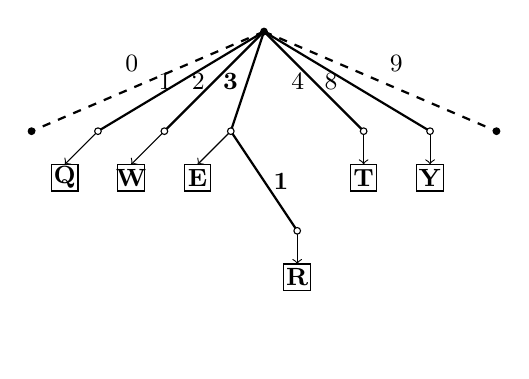
\begin{tikzpicture}[scale=1.2]

\newcommand\Y{-30};
\newcommand\ADDY{-10};

  %% node to node
  \small
  \draw[dashed,thick] (0pt,0pt) -- node[anchor=south east]{0} (-70pt,-30pt);
  \draw[thick] (0pt,0pt) -- node[anchor=east]{1} (-50pt,-30pt); %% Q
  \draw[thick] (0pt,0pt) -- node[anchor=east]{2} (-30pt,-30pt); %% W
  \draw[thick] (0pt,0pt) -- node[anchor=east]{\textbf{3}} (-10pt,-30pt); %% E
  \draw[thick] (0pt,0pt) -- node[anchor=east]{4} ( 30pt,-30pt); %% T
  \draw[thick] (0pt,0pt) -- node[anchor=east]{8} ( 50pt,-30pt); %% Y
  \draw[dashed,thick] (0pt,0pt) -- node[anchor=south west]{9} ( 70pt,-30pt);

  \draw[thick] (-10pt,-30pt) -- node[anchor=west]{\textbf{1}} ( 10pt,-60pt); %% R
%  \draw[thick] (-10pt,-30pt) -- node[anchor=west]{\textbf{0}} (-10pt,-60pt);
%  \draw[thick] (-10pt,-60pt) -- node[anchor=east]{\textbf{X}} (  0pt,-90pt); %% ?


  %% node to element
  \draw[->] (-50pt,\Y pt) -- (-60pt, \ADDY +\Y pt);
  \draw[->] (-30pt,\Y pt) -- (-40pt, \ADDY +\Y pt);
  \draw[->] (-10pt,\Y pt) -- (-20pt, \ADDY +\Y pt);
  \draw[->] ( 30pt,\Y pt) -- ( 30pt, \ADDY +\Y pt);
  \draw[->] ( 50pt,\Y pt) -- ( 50pt, \ADDY +\Y pt);

  \draw[->] ( 10pt,2 * \Y pt) -- ( 10pt, \ADDY + 2 * \Y pt);
%  \draw[->] (  0pt,3 * \Y pt) -- (  0pt, \ADDY + 3 * \Y pt);

  %% nodes
  \draw[fill=black] ( 0pt,  0pt) circle (1pt); 
  \draw[fill=black] (-70pt, -30pt) circle (1pt); 
  \draw[fill=white] (-50pt, -30pt) circle (1pt); %% Q
  \draw[fill=white] (-30pt, -30pt) circle (1pt); %% W
  \draw[fill=white] (-10pt, -30pt) circle (1pt); %% E
  \draw[fill=white] ( 30pt, -30pt) circle (1pt); %% T
  \draw[fill=white] ( 50pt, -30pt) circle (1pt); %% Y
  \draw[fill=black] ( 70pt, -30pt) circle (1pt);

%  \draw[fill=white] (-10pt, 2 * \Y pt) circle (1pt); %% R
  \draw[fill=white] ( 10pt, 2 * \Y pt) circle (1pt); %% x
%  \draw[fill=white] (  0pt, 3 * \Y pt) circle (1pt); %% ?

  %% elements
  \draw[fill=white](-60pt,-4 + \ADDY + \Y pt)
  node{\textbf{Q}} +(-4pt,-4pt) rectangle +(4pt,4pt) ; %% Q
  \draw[fill=white](-40pt,-4 + \ADDY + \Y pt)
  node{\textbf{W}} +(-4pt,-4pt) rectangle +(4pt,4pt) ; %% W
  \draw[fill=white](-20pt,-4 + \ADDY + \Y pt)
  node{\textbf{E}} +(-4pt,-4pt) rectangle +(4pt,4pt) ; %% E
  \draw[fill=white]( 30pt,-4 + \ADDY + \Y pt)
  node{\textbf{T}} +(-4pt,-4pt) rectangle +(4pt,4pt) ; %% T
  \draw[fill=white]( 50pt,-4 + \ADDY + \Y pt)
  node{\textbf{Y}} +(-4pt,-4pt) rectangle +(4pt,4pt) ; %% Y

  \draw[fill=white]( 10pt,-4 + \ADDY + 2 * \Y pt)
  node{\textbf{R}} +(-4pt,-4pt) rectangle +(4pt,4pt) ; %% R
%  \draw[fill=white](  0pt,-4 + \ADDY + 3 * \Y pt)
%  node{\textbf{?}} +(-4pt,-4pt) rectangle +(4pt,4pt) ; %% ?
  \draw(0, -8+\ADDY+ 2.6*\Y pt);

\end{tikzpicture}
}
  \hspace{20pt}
  \subfloat[Les désambiguateurs interviennent lorsqu'un chemin identique a été
  alloué]
  [\label{repl:fig:disexample}L'arbre utilise les désambiguateur afin de
  maintenir un état équivalent, même en présence d'insertions concurrentes ayant
  résulté en des chemins identiques. Par souci de simplicité, seuls les
  désambiguateurs des caractères \texttt{E}, \texttt{R}, et \texttt{T}
  sont affichés.]
  {\begin{tikzpicture}[scale=1.2]

\newcommand\Y{-30};
\newcommand\ADDY{-10};

  %% node to node
  \small
  \draw[dashed,thick] (0pt,0pt) -- node[anchor=south east]{0} (-70pt,\Y pt);
  \draw[thick] (0pt,0pt) -- node[anchor=east]{1} (-50pt, \Y pt); %% Q
  \draw[thick] (0pt,0pt) -- node[anchor=east]{2} (-30pt, \Y pt); %% W
  \draw[thick,color=darkblue] (0pt,0pt)
  -- node[anchor=east]{\DARKBLUE{\textbf{3}}} (  10pt, \Y pt); %% E R
  \draw[thick,color=darkblue] (10pt,\Y pt)
  -- node[anchor=east]{\DARKBLUE{\textbf{1}}} ( 15pt, 2*\Y pt); %% T
  \draw[thick] (0pt,0pt) -- node[anchor=east]{8} ( 50pt, \Y pt); %% Y
  \draw[dashed,thick] (0pt,0pt) -- node[anchor=south west]{9} ( 70pt, \Y pt);

  %% node to element
  \draw[->] (-50pt,\Y pt) -- (-50pt, \ADDY +\Y pt);
  \draw[->] (-30pt,\Y pt) -- (-30pt, \ADDY +\Y pt);
  \draw[->] (  10pt,\Y pt) -- (-10pt, \ADDY +\Y pt);
  \draw[->] (  10pt,\Y pt) -- ( 30pt, \ADDY +\Y pt);
  \draw[->] (  15pt,2*\Y pt) -- ( 15pt, \ADDY + 2*\Y pt);
  \draw[->] ( 50pt,\Y pt) -- ( 50pt, \ADDY +\Y pt);

  %% element to desambiguator
  \draw[<->,densely dotted](-50pt,-8+\ADDY + \Y pt)--(-50pt,2.75*\ADDY+\Y pt);
  \draw[<->,densely dotted](-30pt,-8+\ADDY + \Y pt)--(-30pt,2.75*\ADDY+\Y pt);
  \draw[<->,densely dotted, thick](-10pt,-8+\ADDY + \Y pt)--(-10pt,2.6*\ADDY+\Y pt);
  \draw[<->,densely dotted, thick](15pt,-8+\ADDY + 2*\Y pt)--(15pt,2.6*\ADDY+2*\Y pt);
  \draw[<->,densely dotted, thick]( 30pt,-8+\ADDY + \Y pt)--( 30pt,2.6*\ADDY+\Y pt);
  \draw[<->,densely dotted]( 50pt,-8+\ADDY + \Y pt)--( 50pt,2.75*\ADDY+\Y pt);

  %% nodes
  \draw[fill=black] ( 0pt, 0 pt) circle (1pt); 
  \draw[fill=black] (-70pt, \Y pt) circle (1pt); 
  \draw[fill=white] (-50pt, \Y pt) circle (1pt); %% Q
  \draw[fill=white] (-30pt, \Y pt) circle (1pt); %% W
  \draw[fill=white] ( 10pt, \Y pt) circle (1pt); %% E
  \draw[fill=white] ( 15pt, 2*\Y pt) circle (1pt); %% T
  \draw[fill=white] ( 50pt, \Y pt) circle (1pt); %% Y
  \draw[fill=black] ( 70pt, \Y pt) circle (1pt);

  %% desambiguator
  \draw[fill=gray!20] (-50pt,-2.5+2.75*\ADDY+\Y pt)
  +(-2.5pt,-2.5pt) rectangle +(2.5pt,2.5pt);
  \draw[fill=gray!20] (-30pt,-2.5+2.75*\ADDY+\Y pt)
  +(-2.5pt,-2.5pt) rectangle +(2.5pt,2.5pt);
  \draw[fill=gray!20] (-10pt,-2.5+2.75*\ADDY+\Y pt)
  node{\DARKBLUE{$\langle c_1,\, 3\rangle$}}
  +(-12pt,-4pt) rectangle +(12pt,4pt);
  \draw[fill=gray!20] ( 15pt,-2.5+2.75*\ADDY+2*\Y pt)
  node{\DARKBLUE{$\langle c_1,\, 3\rangle\langle c_1,\,5\rangle$}}
  +(-26pt,-4pt) rectangle +(26pt,4pt);
  \draw[fill=gray!20] ( 30pt,-2.5+2.75*\ADDY+\Y pt)
  node{\DARKBLUE{$\langle c_2,\, 1\rangle$}}
  +(-12pt,-4pt) rectangle +(12pt,4pt);
  \draw[fill=gray!20] ( 50pt,-2.5+2.75*\ADDY+\Y pt)
  +(-2.5pt,-2.5pt) rectangle +(2.5pt,2.5pt);

  %% elements
  \draw[fill=white](-50pt,-4 + \ADDY + \Y pt)
  node{\textbf{Q}} +(-4pt,-4pt) rectangle +(4pt,4pt) ; %% Q
  \draw[fill=white](-30pt,-4 + \ADDY + \Y pt)
  node{\textbf{W}} +(-4pt,-4pt) rectangle +(4pt,4pt) ; %% W
  \draw[fill=white](- 10pt,-4 + \ADDY + \Y pt)
  node{\textbf{E}} +(-4pt,-4pt) rectangle +(4pt,4pt) ; %% E
  \draw[fill=white]( 15pt,-4 + \ADDY + 2*\Y pt)
  node{\textbf{R}} +(-4pt,-4pt) rectangle +(4pt,4pt) ; %% R
  \draw[fill=white]( 30pt,-4 + \ADDY + \Y pt)
  node{\textbf{T}} +(-4pt,-4pt) rectangle +(4pt,4pt) ; %% T
  \draw[fill=white]( 50pt,-4 + \ADDY + \Y pt)
  node{\textbf{Y}} +(-4pt,-4pt) rectangle +(4pt,4pt) ; %% Y

  
  % \begin{scope}[shift={(20pt, 2.5*\Y pt)}]    
  %   \draw[fill=white](0,0)node{\textbf{E}} +(-4pt, -4pt) rectangle +(4pt, 4pt);
  %   \scriptsize
  %   \draw (4pt, 0)node[anchor=west]{element};
  %   \draw[fill=gray!20] (0,\ADDY pt) +(-2.5pt, -2.5pt)rectangle+(2.5pt, 2.5pt);
  %   \draw (3pt, \ADDY pt) node[anchor=west]{disambiguator};
  % \end{scope}
  %% spacing
  \draw(0, -8+\ADDY+ 2.6*\Y pt);

\end{tikzpicture}
}
  \caption[Arbres contenant une séquence répliquée]
  {Arbres contenant la séquence \texttt{QWERTY}.}
\end{figure}

La figure~\ref{repl:fig:treeexample} montre l'arbre d'arité maximale 10
représentant la séquence. Un auteur insère les caractères \texttt{QWTY} les uns
à la suite des autres. Les chemins en résultant sont [1], [2], [4] et [8]
respectivement. L'insertion du caractère \texttt{E} entre les paires
$\langle [2],\, \texttt{W} \rangle$ et $\langle [4],\, \texttt{T} \rangle$
engendre la paire suivante : $\langle [3],\, \texttt{E} \rangle$. Pour insérer
le caractère \texttt{R}, l'arbre doit être agrandi afin d'accueillir le nouveau
chemin entre \texttt{E} et \texttt{T}. Le chemin en résultant est [3.1]. Insérer
un nouveau caractère entre \texttt{E} et \texttt{R} résulterait en une autre
augmentation de la profondeur de l'arbre. Le chemin serait [3.0.$X$] où
$0<X<10$. L'ordre total $(\mathcal{P},\, <_\mathcal{P})$ permet de retrouver la
séquence \texttt{QWERTY}.


\paragraph{Désambiguation des cas concurrents.}

L'ordre des chemins $(\mathcal{P},\, <_\mathcal{P})$ est un ordre total
lorsqu'un seul auteur écrit. Toutefois, cela devient un ordre partiel lorsque
plusieurs auteurs sont impliqués dans l'édition. Par exemple, si deux auteurs
insèrent un caractère au même endroit dans le document, au même moment, le même
chemin pour les deux caractères risque d'être alloué. Dans ce cas, l'ordre des
caractères n'est pas strictement défini et peut rompre la propriété de
convergence des répliques. Les désambiguateurs utilisent des marqueurs unique de
manière globale pour fournir un ordre total même en présence d'édition
concurrente. Ces marqueurs sont généralement constitués d'un identifiant de site
unique associé à une horloge de Lamport~\cite{lamport1978time}. Chaque paire
$\langle chemin,\, element \rangle$ est associée à un désambiguateur.

Soit l'ensemble des identifiants $\mathcal{I}$ composés tels que
$\mathcal{I} : \mathcal{P} \times \mathcal{A} \times \mathcal{D}$. La
composition de l'ordre partiel $(\mathcal{P},\,<_\mathcal{P})$ et l'ordre total
des désambiguateurs $(\mathcal{D},\, <_\mathcal{D})$ permet d'ordonner les
éléments de la séquence de manière identique quelle que soit la réplique.

La figure~\ref{repl:fig:disexample} montre l'arbre contenant 6 éléments mais
seulement 5 chemins distincts. Tout d'abord, le premier collaborateur $c_1$
insère \texttt{QW}. Ensuite, les collaborateurs $c_1$ et $c_2$ insèrent en
concurrence les caractères \texttt{E} et \texttt{T}, respectivement. Dans les
deux cas, le chemin en résultant est $[3]$. Pour résoudre cette ambiguïté, le
désambiguateur $\langle c_1,\, 3 \rangle$ est associé au caractère \texttt{E};
le désambiguateur $\langle c_2,\, 1 \rangle$ est associé au caractère
\texttt{T}. Recouvrer l'ordre des éléments consiste simplement à comparer, à
chaque niveau de l'arbre, le chemin du niveau, puis l'identifiant de la
réplique, puis l'horloge. Dans cet exemple, le caractère \texttt{E} précède le
caractère \texttt{T} car $c_1< c_2$. Ensuite, le collaborateur $c_1$ insère
\texttt{Y} à la fin de la séquence. Enfin, il insère \texttt{R} entre \texttt{E}
et \texttt{T}. Puisque ces derniers ont un chemin identique, l'espace est
insuffisant entre ces deux chemins pour insérer un nouveau caractère. La
profondeur de l'arbre doit augmenter. La fonction d'allocation doit choisir un
chemin $[3.X]$ tel que $0<X<10$. En copiant le désambiguateur de \texttt{E} au
premier niveau, cela assure que le nouvel identifiant suivra celui du caractère
\texttt{E} et précédera celui du caractère \texttt{T}. Il est important de noter
que les collaborateurs ne choisissent pas les désambiguateurs. Ainsi, la
séquence de cet exemple aurait pu être \texttt{QWTREY} auquel cas une correction
aurait été nécessaire. De plus, la complexité spatiale de ces désambiguateurs
est bornée par leur chemin respectif. Par conséquent, le reste de ce chapitre se
concentre sur ces chemins.

% Nous définissons le modèle suivant : le CRDT est un arbre $T$ initialisé vide
% équippé des opérations d'insertion $\textsc{insert}$ et de suppression
% $\textsc{delete}$. Un identifiant dans $\mathcal{I}$ contient un chemin dans
% $\mathcal{P}$, un désambiguateur dans $\mathcal{D}$, et un élément dans
% l'alphabet $\mathcal{A}$. L'union des identifiants non supprimés crée l'arbre
% $T$ où chaque noeud possède au plus un élément.  En utilisant un ordre total
% $(\mathcal{I},\, <_\mathcal{I})$, l'arbre est transformé en séquence d'éléments.

% Un chemin est une liste d'entiers dont la taille borne celle du désambiguateur :
% une liste constituée de paires avec l'identifiant unique du serveur hébergeant
% la réplique, et un compteur local à cette réplique (cf. l'exemple des CRDTs pour
% compteurs §\ref{repl:subsubsec:crdts}). La complexité de l'identifiant dépend donc
% essentiellement de l'allocation du chemin dans l'arbre.

\paragraph{Choisir le bon chemin.} La composante la plus critique des approches
pour les séquences où les identifiants sont de taille variable consiste à
choisir les chemins. L'algorithme~\ref{repl:algo:general} montre les
instructions générales de telles approches. Il divise les opérations --
insertion et suppression -- entre la partie locale et la partie distante du
schéma de réplication optimiste. Le cœur de l'algorithme est situé dans la
partie locale de l'opération d'insertion où le chemin et le désambiguateur
doivent être créés. La fonction \textsc{convert2Path} se débarrasse de la partie
désambiguateur des identifiants en argument pour n'en garder que les chemins --
transformés si nécessaire. Lorsqu'il n'y a pas de marques d'opérations
concurrentes, les chemins sont simplement retournés tels quels. Dans le cas
contraire, cette fonction convertit les identifiants en chemins préservant
l'ordre $(\mathcal{P}, <_\mathcal{P})$. Par exemple, dans la
figure~\ref{repl:fig:disexample}, le résultat de l'appel à la fonction
\textsc{convert2Path} avec les identifiants du caractère \texttt{E} et du
caractère \texttt{T} est la paire $\langle [3.0],\, [3.9] \rangle$. La fonction
\textsc{allocPath} alloue un nouveau chemin entre ces bornes. \textsc{allocDis}
décore le chemin pour garantir que l'identifiant -- en tant que composition d'un
chemin, d'un élément, et d'un désambiguateur -- est bien positionné entre les
identifiants qui ont servi à le créer selon la relation d'ordre
$(\mathcal{I},\, <_\mathcal{I})$.

\begin{algorithm}[h]
  
\small
\algrenewcommand{\algorithmiccomment}[1]{\hskip2em$\rhd$ #1}

\newcommand{\comment}[1]{$\rhd$ #1}


\algblockdefx[initially]{initially}{endInitially}
  [0] {\textbf{INITIALLY:}} 

\algblockdefx[local]{local}{endLocal}
  [0] {\textbf{LOCAL UPDATE:}}

\algsetblockdefx[received]{received}{endReceived}
  {65535}{}
  [0] {\textbf{RECEIVED UPDATE:}}

\algblockdefx[onInsert]{onLocal}{endOnLocal}
  [0] {\textbf{on} insert ($previous \in \mathcal{I},\,\alpha \in \mathcal{A},\,
   next\in\mathcal{I}$):}
  [0] {\textbf{on} delete ($i \in \mathcal{I}$):} 

\algsetblockdefx[onRemote]{onRemote}{endOnRemote}
  {65535}{}
  [0] {\textbf{on} insert ($i\in\mathcal{I}$):
    \hfill\comment{\textbf{une fois} par identifiant}}
  [0] {\textbf{on} delete ($i\in\mathcal{I}$):
    \hfill\comment{\textbf{après} l'exécution de \textsc{insert}($i$)}} 

\newcommand{\LINEFOR}[2]{%
  \algorithmicfor\ {#1}\ \algorithmicdo\ {#2} %
  }

\newcommand{\LINEIFTHEN}[2]{%
  \algorithmicif\ {#1}\ \algorithmicthen\ {#2} %
  }

\newcommand{\INDSTATE}[1][1]{\State\hspace{\algorithmicindent}}

\begin{algorithmic}[1]
  \Statex
  \initially
    \State $T \leftarrow \varnothing$;
    \hfill \comment{CRDT conçue pour les séquences}
  \endInitially
  
  \local
    \onLocal
    \State \textbf{let}
    $\langle p,\, q \rangle \leftarrow \textsc{convert2Path}(previous,\, next)$;
    \State \textbf{let}
    $newPath \leftarrow \DARKBLUE{\textsc{allocPath}(p,\,q)}$; \label{line:allocpath}
    \State \textbf{let} 
    $newDis \leftarrow \textsc{allocDis}(p,\, newPath,\, q)$; \label{line:allocdes}
    \State $\textsc{broadcast}(\text{'insert'},\,
    \langle newPath,\, \alpha,\, newDis \rangle)$;
    \endOnLocal
    \INDSTATE $\textsc{broadcast}(\text{'delete'},\,i)$;
  \endLocal
  
  \received
    \onRemote
    \State $T \leftarrow T \cup i$;
    \endOnRemote
    \INDSTATE $T \leftarrow T\, \backslash\, i$; 
  
\end{algorithmic}

  \caption[Séquences avec identifiants de taille variable]
  {\label{repl:algo:general}Séquences avec identifiants de taille variable.}
\end{algorithm}

La fonction \textsc{allocPath} choisit le chemin dans l'arbre entre deux autres
chemins $p$ et $q$ tels que $p$ précède $q$ (i.e. $p <_\mathcal{P} q$).  Le
nouveau chemin $n$ est positionné entre ces bornes (i.e.
$p <_\mathcal{P} n <_\mathcal{P} q$). La fonction \textsc{allocPath} doit
choisir parmi les plus petits chemins disponibles afin de conserver de bonnes
performances.

\begin{figure}
  \begin{center}
  \subfloat[Allocation quasi-optimale]
  [\label{repl:fig:allocpathexampleA}Allocation presque optimale]
  {\begin{tikzpicture}[scale=1.2]

  %% node to node
  \small
  \draw[dashed, thick] (0pt,0pt) -- node[anchor=south east]{0} (-70pt,-40pt);
  \draw[thick] (0pt,0pt) -- node[anchor=east]{\DARKBLUE{1}} (-50pt,-40pt);
  \draw[thick] (0pt,0pt) -- node[anchor=east]{\DARKBLUE{2}} (-30pt,-40pt);
  \draw[thick] (0pt,0pt) -- node[anchor=east]{\DARKBLUE{3}} (-10pt,-40pt);
  \draw[thick] (0pt,0pt) -- node[anchor=west]{\DARKBLUE{4}} ( 10pt,-40pt);
  \draw[thick] (0pt,0pt) -- node[anchor=west]{\DARKBLUE{5}} ( 30pt,-40pt);
  \draw[thick] (0pt,0pt) -- node[anchor=west]{\DARKBLUE{6}} ( 50pt,-40pt);
  \draw[dashed, thick] (0pt,0pt) -- node[anchor=south west]{9} ( 70pt,-40pt);

  %% node to element
  \draw[->] (-50pt,-40pt) -- (-50pt,-50pt);
  \draw[->] (-30pt,-40pt) -- (-30pt,-50pt);
  \draw[->] (-10pt,-40pt) -- (-10pt,-50pt);
  \draw[->] ( 10pt,-40pt) -- ( 10pt,-50pt);
  \draw[->] ( 30pt,-40pt) -- ( 30pt,-50pt);
  \draw[->] ( 50pt,-40pt) -- ( 50pt,-50pt);

  %% element to desambiguator
  \draw[->,densely dashdotted] ( -50pt,-58pt) -- ( -50pt,-68.5pt);
  \draw[->,densely dashdotted] ( -30pt,-58pt) -- ( -30pt,-68.5pt);
  \draw[->,densely dashdotted] ( -10pt,-58pt) -- ( -10pt,-68.5pt);
  \draw[->,densely dashdotted] (  10pt,-58pt) -- (  10pt,-68.5pt);
  \draw[->,densely dashdotted] (  30pt,-58pt) -- (  30pt,-68.5pt);
  \draw[->,densely dashdotted] (  50pt,-58pt) -- (  50pt,-68.5pt);

  \draw[fill=black] (  0pt,  0pt) circle (1pt);
  \draw[fill=black] (-70pt,-40pt) circle (1pt);
  \draw[fill=white] (-50pt,-40pt) circle (1pt);
  \draw[fill=white] (-30pt,-40pt) circle (1pt);
  \draw[fill=white] (-10pt,-40pt) circle (1pt);
  \draw[fill=white] ( 10pt,-40pt) circle (1pt);
  \draw[fill=white] ( 30pt,-40pt) circle (1pt);
  \draw[fill=white] ( 50pt,-40pt) circle (1pt);
  \draw[fill=black] ( 70pt,-40pt) circle (1pt);

  %% elements
  \draw[fill=white](-50pt,-54pt)
  node{\textbf{Q}}+(-4pt,-4pt)rectangle+(4pt,4pt) ;
  \draw[fill=white](50pt,-54pt)
  node{\textbf{Y}} +(-4pt,-4pt) rectangle +(4pt,4pt) ;
  \draw[fill=white]( 10pt,-54pt)
  node{\textbf{R}} +(-4pt,-4pt) rectangle +(4pt,4pt) ;
  \draw[fill=white] ( -30pt,-54pt)
  node{\textbf{W}} +(-4pt,-4pt) rectangle +(4pt,4pt) ;
  \draw[fill=white] ( -10pt,-54pt)
  node{\textbf{E}} +(-4pt,-4pt) rectangle +(4pt,4pt) ;
  \draw[fill=white]( 30pt,-54pt)
  node{\textbf{T}} +(-4pt,-4pt) rectangle +(4pt,4pt) ;

  %% desambiguator
  \draw[fill=gray!20] (-50pt,-71pt) +(-2.5pt,-2.5pt) rectangle +(2.5pt,2.5pt);
  \draw[fill=gray!20] (-30pt,-71pt) +(-2.5pt,-2.5pt) rectangle +(2.5pt,2.5pt);
  \draw[fill=gray!20] (-10pt,-71pt) +(-2.5pt,-2.5pt) rectangle +(2.5pt,2.5pt);
  \draw[fill=gray!20] ( 10pt,-71pt) +(-2.5pt,-2.5pt) rectangle +(2.5pt,2.5pt);
  \draw[fill=gray!20] ( 30pt,-71pt) +(-2.5pt,-2.5pt) rectangle +(2.5pt,2.5pt);
  \draw[fill=gray!20] ( 50pt,-71pt) +(-2.5pt,-2.5pt) rectangle +(2.5pt,2.5pt);

  %% insertion order
  \draw[->,dashed, color=darkblue] (-50pt, -90pt)
  -- node[anchor=north]{\DARKBLUE{ordre d'insertion}} (50pt, -90pt);

\end{tikzpicture}
}
  \hspace{30pt}
  \subfloat[Allocation pire-cas]
  [\label{repl:fig:allocpathexampleB}Allocation pire cas]
  {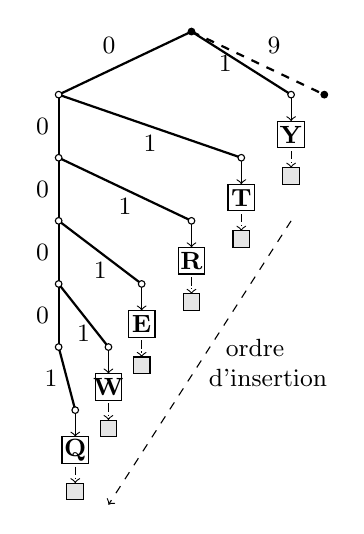
\begin{tikzpicture}[scale=1.2]

\newcommand\Y{-19}
\newcommand\ADDY{-8}

  %% node to node
  \small
  \draw[thick] (0pt,0pt) -- node[anchor=south east]{\DARKBLUE{0}} (-40pt,\Y pt);
  \draw[thick] (0pt,0pt) -- node[anchor=east]{1} (30pt, \Y pt); %% Y
  \draw[thick] (-40pt, \Y pt) -- node[anchor=north]{1} (15pt, 2 * \Y pt); %% T
  \draw[thick] (-40pt, \Y pt) -- node[anchor=east]{\DARKBLUE{0}} (-40pt, 2 * \Y pt); %% 0
  \draw[thick] (-40pt, 2*\Y pt) -- node[anchor=north]{1} (0pt, 3 * \Y pt); %% R
  \draw[thick] (-40pt, 2*\Y pt)-- node[anchor=east]{\DARKBLUE{0}}(-40pt, 3 * \Y pt); %% 0
  \draw[thick] (-40pt, 3*\Y pt) -- node[anchor=north]{1}(-15pt,4 * \Y pt); %% E
  \draw[thick] (-40pt, 3*\Y pt) -- node[anchor=east]{\DARKBLUE{0}}(-40pt,4 * \Y pt); %% 0
  \draw[thick] (-40pt, 4*\Y pt) -- node[anchor=north]{1}(-25pt,5 * \Y pt); %% W
  \draw[thick] (-40pt, 4*\Y pt) -- node[anchor=east]{\DARKBLUE{0}}(-40pt,5 * \Y pt); %% 0
  \draw[thick] (-40pt, 5*\Y pt) -- node[anchor=east]{\DARKBLUE{1}}(-35pt,6 * \Y pt); %% Q

  \draw[dashed, thick] (0pt,0pt) -- node[anchor=south west]{9} (40pt,\Y pt);

  %% node to element
  \draw[->] ( 30pt, \Y pt) -- ( 30pt, \ADDY + \Y pt); %% Y
  \draw[->] ( 15pt, 2* \Y pt) -- ( 15pt, \ADDY + 2 *\Y pt); %% T
  \draw[->] (  0pt, 3 *\Y pt) -- (  0pt, \ADDY + 3 *\Y pt); %% R
  \draw[->] (-15pt, 4 *\Y pt) -- ( -15pt, \ADDY + 4 *\Y pt); %% E
  \draw[->] (-25pt, 5 *\Y pt) -- ( -25pt, \ADDY + 5 *\Y pt); %% W
  \draw[->] (-35pt, 6 *\Y pt) -- ( -35pt, \ADDY + 6 *\Y pt); %% Q

  %% element to desambiguator
  \draw[->,densely dashdotted]
  ( 30pt, \ADDY + \Y pt) -- ( 30pt,2.75*\ADDY+\Y pt); %% Y
  \draw[->,densely dashdotted]
  ( 15pt, \ADDY + 2* \Y pt) -- ( 15pt,2.75*\ADDY+ 2* \Y pt); %% T
  \draw[->,densely dashdotted]
  ( 0pt, \ADDY + 3* \Y pt) -- (  0pt,2.75*\ADDY+ 3* \Y pt); %% R
  \draw[->,densely dashdotted]
  ( -15pt, \ADDY + 4 *\Y pt) -- ( -15pt,2.75*\ADDY+ 4* \Y pt); %% E
  \draw[->,densely dashdotted]
  ( -25pt, \ADDY + 5 *\Y pt) -- ( -25pt,2.75*\ADDY+ 5*\Y pt); %% W
  \draw[->,densely dashdotted]
  ( -35pt, \ADDY + 6* \Y pt) -- ( -35pt,2.75*\ADDY+ 6*\Y pt); %% Q

  %% node
  \draw[fill=black] (0pt,0pt) circle (1pt); %% rooot
  \draw[fill=white] ( 30pt, \Y pt) circle (1pt); %% Y
  \draw[fill=white] (-40pt, \Y pt) circle (1pt); %% 0
  \draw[fill=white] ( 15 pt, 2 * \Y pt) circle (1pt); %% T
  \draw[fill=white] (-40pt, 2 * \Y pt) circle (1pt); %% 0
  \draw[fill=white] (  0 pt, 3 * \Y pt) circle (1pt); %% R
  \draw[fill=white] (-40pt, 3 * \Y pt) circle (1pt); %% 0
  \draw[fill=white] (-15 pt, 4 * \Y pt) circle (1pt); %% E
  \draw[fill=white] (-40pt, 4 * \Y pt) circle (1pt); %% 0
  \draw[fill=white] (-25 pt, 5 * \Y pt) circle (1pt); %% W
  \draw[fill=white] (-40pt, 5 * \Y pt) circle (1pt); %% 0
  \draw[fill=white] (-35 pt, 6 * \Y pt) circle (1pt); %% Q

  \draw[fill=black] ( 40pt, \Y pt) circle (1pt);


  %% elements
  \draw[fill=white] ( 30pt, -4 + \ADDY + \Y pt)
  node{\textbf{Y}} +(-4pt,-4pt) rectangle +(4pt,4pt) ; %% Y
  \draw[fill=white] ( 15pt, -4 + \ADDY +  2 *\Y pt)
  node{\textbf{T}} +(-4pt,-4pt) rectangle +(4pt,4pt) ; %% T
  \draw[fill=white] (  0pt, -4 + \ADDY +  3* \Y pt)
  node{\textbf{R}} +(-4pt,-4pt) rectangle +(4pt,4pt) ; %% R
  \draw[fill=white] (-15pt, -4 + \ADDY + 4 *\Y pt)
  node{\textbf{E}} +(-4pt,-4pt) rectangle +(4pt,4pt) ; %% E
  \draw[fill=white] (-25pt, -4 + \ADDY + 5 * \Y pt)
  node{\textbf{W}} +(-4pt,-4pt) rectangle +(4pt,4pt) ; %% W
  \draw[fill=white] (-35pt, -4 + \ADDY + 6 *\Y pt)
  node{\textbf{Q}} +(-4pt,-4pt) rectangle +(4pt,4pt) ; %% Q

  %% desambiguator
  \draw[fill=gray!20]( 30pt, -2.5 + 2.75 * \ADDY + \Y pt)
  +(-2.5pt,-2.5pt) rectangle +(2.5pt,2.5pt);
  \draw[fill=gray!20]( 15pt, -2.5 + 2.75 * \ADDY +2 *\Y pt)
  +(-2.5pt,-2.5pt) rectangle +(2.5pt,2.5pt);
  \draw[fill=gray!20](  0pt, -2.5 + 2.75 * \ADDY + 3*\Y pt)
  +(-2.5pt,-2.5pt) rectangle +(2.5pt,2.5pt);
  \draw[fill=gray!20](-15pt, -2.5 + 2.75 * \ADDY +4*\Y pt )
  +(-2.5pt,-2.5pt) rectangle +(2.5pt,2.5pt);
  \draw[fill=gray!20](-25pt, -2.5 + 2.75 * \ADDY + 5*\Y pt)
  +(-2.5pt,-2.5pt) rectangle +(2.5pt,2.5pt);
  \draw[fill=gray!20](-35pt, -2.5 + 2.75 * \ADDY +6*\Y pt) 
  +(-2.5pt,-2.5pt) rectangle +(2.5pt,2.5pt);

  %% insertion order
  \draw[->,dashed] (30pt, 3 * \Y pt) -- node[anchor=west,align=left]
  {\ \ ordre\\ d'insertion} (-25pt, 7.5 * \Y pt);

\end{tikzpicture}
}
  \end{center}
  \caption[Une stratégie d'allocation contre les comportements d'édition] {Une
    même stratégie d'allocation face à des comportements d'édition différents.}
\end{figure}

Les figures~\ref{repl:fig:allocpathexampleA} et~\ref{repl:fig:allocpathexampleB}
illustrent les difficultés rencontrées lors de l'allocation des chemins
composant les identifiants. Dans les deux cas, la fonction d'allocation utilise
la stratégie suivante : la branche la plus à gauche avec la plus petite
profondeur possible. Dans les deux cas, la séquence finale est
\texttt{QWERTY}. Toutefois, les lettres ne sont pas insérées dans un ordre
identique. Dans le premier cas, la lettre \texttt{Q} est insérée à l'indice 0,
suivie de la lettre \texttt{W} à l'indice 1, suivie de la lettre \texttt{E} à
l'indice 2, etc.  Dans le second cas, la lettre \texttt{Y} est insérée à
l'indice 0, suivie de \texttt{T} à l'indice 0 qui, par effet de bord, décale le
\texttt{Y} à l'indice 1. La séquence en résultant est donc
\texttt{TY}. L'insertion de \texttt{R} en position 0 décale toutes lettres de
droite, etc.

Dans le premier cas (cf. figure~\ref{repl:fig:allocpathexampleA}), l'opération
d'insertion (\texttt{Q}, 0) est transformée en \textsc{insert}($\vdash$,
\texttt{Q}, $\dashv$). Par conséquent, le chemin doit être alloué entre les
bornes virtuelles [0] et [9]. Puisque la stratégie d'allocation consiste à
réserver la branche la plus à gauche et de plus petite taille, le chemin
résultant est [1]. Ensuite, l'opération (\texttt{W}, 1) est transformée en
\textsc{insert}($i_Q$, \texttt{W}, $\dashv$) résultant en le chemin [2], etc.
Dans ce cas, la profondeur de l'arbre n'augmente jamais. À cet égard, la
stratégie employée est très efficace. Cependant, elle n'est pas totalement
optimale puisque l'arbre est prévu pour accueillir 8 identifiants alors que
seulement 6 sont alloués.

Dans le second cas (cf. figure~\ref{repl:fig:allocpathexampleB}), l'opération
d'insertion (\texttt{Y}, 0) est transformée en \textsc{insert}($\vdash$,
\texttt{Y}, $\dashv$) dont le résultat est le chemin [1]. Lors de l'insertion
(\texttt{T}, 0), un chemin est requis entre la borne virtuelle du début de
séquence [0] et la borne du caractère \texttt{Y} : [1]. Ainsi, la profondeur du
chemin doit augmenter de telle sorte que le nouvel identifiant muni de l'ordre
total $(\mathcal{I},\,<_\mathcal{I})$ soit placé entre les deux. Considérons un
ordre lexicographique, le chemin résultant est [0.$X$] où $X$ est choisi entre 0
et 10. Suivant la stratégie, le chemin est [0.1] pour la lettre \texttt{T}. Puis
[0.0.1] pour la lettre \texttt{R}, etc. La taille des chemins alloués augmente
très rapidement.  La stratégie d'allocation s'avère inefficace dans ce cas.

Cet exemple montre à quel point l'ordre d'insertion des éléments affecte la
longueur des chemins alloués. Malheureusement, ni la séquence d'édition, ni sa
taille ne sont connues par avance.  Passer d'indices locaux mutables et optimaux
d'une séquence classique à des identifiants non-mutables de taille variable
d'une séquence répliquée a un coût qu'il convient d'analyser afin de proposer
une fonction d'allocation efficace. Le problème scientifique que l'on souhaite
résoudre est le suivant :

\begin{problem}
  Soit la séquence d'identifiants $s(I)= id_1.id_2\ldots id_I$, et
  $s(I+1) = s(I) \cup \textsc{insert}(p,\, \_,\, n)$ où $p,q \in s(I)$ et
  $p<_\mathcal{I}q$. Soit $|s(I)|$ la taille de la représentation binaire de la
  séquence. La fonction \textsc{insert} doit allouer des identifiants tels que :
  \begin{equation}
    |s(I+1)| - |s(I)| < \mathcal{O}(I)
  \end{equation}
\end{problem}

En d'autres termes, les chemins alloués par la fonction d'allocation
\textsc{allocPath}, principal élément de la fonction \textsc{insert}, doivent
garantir des chemins dont la taille est sous-linéaire par rapport au nombre
d'insertions dans la séquence. Logoot et Treedoc échouent à fournir des
identifiants de taille bornée de cette façon dans les cas d'insertions de gauche
à droite et de droite à gauche. Ces deux approches nécessitent l'exécution
périodique d'un mécanisme de relocalisation des identifiants afin de conserver
de bonnes performances.

La section suivante présente \LSEQ, une fonction d'allocation d'identifiants
dont la taille croît de manière polylogarithmique par rapport au nombre
d'insertions effectuées dans la séquence. Par conséquent, aucun mécanisme
additionnel de relocalisation n'est nécessaire.


%%% Local Variables:
%%% mode: latex
%%% TeX-master: "../../paper"
%%% End:
